\documentclass[fleqn,svgnames,screen,acmsmall]{ml2rcn}

\usepackage{amsthm}
\usepackage{pdfpages}
\usepackage{caption}
\usepackage{pyimport}

\newcommand{\additionalcomment}[1]{\textcolor{blue}{#1}}
\newcommand{\addORCID}[1]{~\href{https://orcid.org/#1}{
\includegraphics[width=1.5ex]{ORCID.png}}}

\newtheorem{theorem}{Theorem}
\newtheorem{definition}{Definition}

\begin{document}

% set up pdf meta data
\hypersetup{%
  pdftitle={The Gracefulness of Graph B(m,n)},
  pdfauthor={Guo Wenfu, translation by Pascal Welke}
  pdfsubject={graph theory, python},
  pdfkeywords={cycle, path, tadpole, graceful graph}
}


\author[G. Wenfu]{Guo Wenfu}
\affiliation{
  \institution{Translation, \additionalcomment{comments}, and \texttt{code} by Pascal Welke \addORCID{0000-0002-2123-3781}}
  \city{Lancaster University Leipzig}
  \state{Germany}
}


\title{\texorpdfstring{The Gracefulness of Graph
\(B(m,n)\)}{The Gracefulness of Graph B(m,n)}}


\begin{abstract}
\textbf{Abstract.} 
In this paper, we shall prove that the graphs
\(B(m,n) = C_{m} \cup P_{n}\) are \textbf{graceful} when \(m \equiv 1\)
or \(2 \pmod 4\), where \(C_{m} = A_{1}A_{2} \ldots A_{m}A_{1}\) and
\(P_{n} = A_{1}B_{1}B_{2} \ldots B_{n}\) (\(m \ge 3, n > 0\)).

\paragraph{Keywords:} {cycle, path, tadpole, graceful graph}
\end{abstract}


\maketitle


\additionalcomment{I have obtained the original Chinese version [\ref{citeoriginal}] of this article with the help of collegues and translated it with the help of Google Gemini as of December 2025. 
I have checked the proof sketches in the translation carefully and have implemented all constructions in Python. 
All functions are named after the respective parts of the original paper and construct a sequence of vertices that are injectively labeled with numbers from $1$ to $m+n$ and a sequence of edges.
As the vertex labeling is injective, I used the labels as node ids.
The code is provided next to the descriptions of the original paper and is available on \href{https://github.com/pwelke/graceful_tadpoles}{github}. }

\section{Introduction}\label{introduction}
 
Let the \textbf{cycle} be \(C_{m} = A_{1}A_{2} \ldots A_{m}A_{1}\) and
the \textbf{path} be \(P_{n} = A_{1}B_{1}B_{2} \ldots B_{n}\). We define
the graph \textbf{\(B(m,n) = C_{m} \cup P_{n}\)} (\(m \ge 3, n > 0\)).

It has been proven in [\ref{cite1}] that \(B(m,n)\) is a \(1\)-graceful graph.
It was also proven that \(B(m,n)\) is a graceful graph when
\(m \equiv 0\) or \(3 \pmod 4\). This paper gives an affirmative answer to the question: ``Is \(B(m,n)\) a graceful graph when
\(m \equiv 1\) or \(2 \pmod 4\) and \(n > 0\)?''.

\begin{definition}[Graceful Labeling]
\label{graceful-graph-definition}
  For a simple graph \(G(V, E)\) we assign non-negative integers \(\varphi(v) \in \{1, 2, \ldots, |E|\}\) to every vertex \(v \in V\) which we call \emph{vertex labels}. 
  We call the value \(L(u, v) = |\varphi(u) - \varphi(v)|\) the \emph{edge label} of the edge \(uv\). 
  A simple graph \(G\) is called a \emph{graceful
  graph} if it is labeled such that: 
  \begin{enumerate}
    % \item The vertex labels are taken from \(I\). 
    \item Different vertices have different vertex labels. 
    \item Different edges have different edge labels.
  \end{enumerate}
\end{definition}

The set of edge labels for a graceful graph is
\(\{1, 2, \ldots, |E|\}\). 
% The paper uses \(N_{1}\) (\(N_{2}\)) to denote the set of all \emph{odd (even) numbers}.

\additionalcomment{The entrypoint to the python code is the following function that constructs a graceful labeling for any tadpole with \(m \equiv 1\) or \(2 \pmod 4\).}

\vspace{0.5\baselineskip}
\pyfunction{../code/graceful_tadpoles.py}{graceful_tadpole}

\section{\texorpdfstring{Case
\(m \equiv 2 \pmod 4\)}{Case m \textbackslash equiv 2 \textbackslash pmod 4}}\label{theorem-1-case-m-equiv-2-pmod-4}

\begin{theorem}
For all \(m \equiv 2 \pmod 4\) and \(n > 0\),
\(B(m,n)\) is a \textbf{graceful graph}.
\end{theorem}

\begin{proof}
Let \(m = 4l + 2\), which implies \(l = \frac{m-2}{4}\).
A graceful labeling for $n=1$ and arbitrary $l>0$ is given in Figure 1 \additionalcomment{with comments and python code in Section~\ref{sec:fig1}}.%Figure 1. 
Similarly, a graceful labeling for $n=2$ and arbitrary $l>0$ is given in Figure 2 \additionalcomment{with comments and python code in Section~\ref{sec:fig2}}. 
% \additionalcomment{Python code to create these graceful labelings is provided in Algorithm~\ref{alg:fig1} and Algorithm~\ref{alg:fig2}.}
For the case \(n \ge 3\) we will construct graceful labelings in Section~\ref{sec:restofthm1}.
\end{proof} 

\vspace{0.5\baselineskip}
\pyfunction{../code/graceful_tadpoles.py}{thm1}

\subsection{Case 1: \(n = 1\)}
\label{sec:fig1}

\begin{minipage}{\textwidth}
\begin{center}
  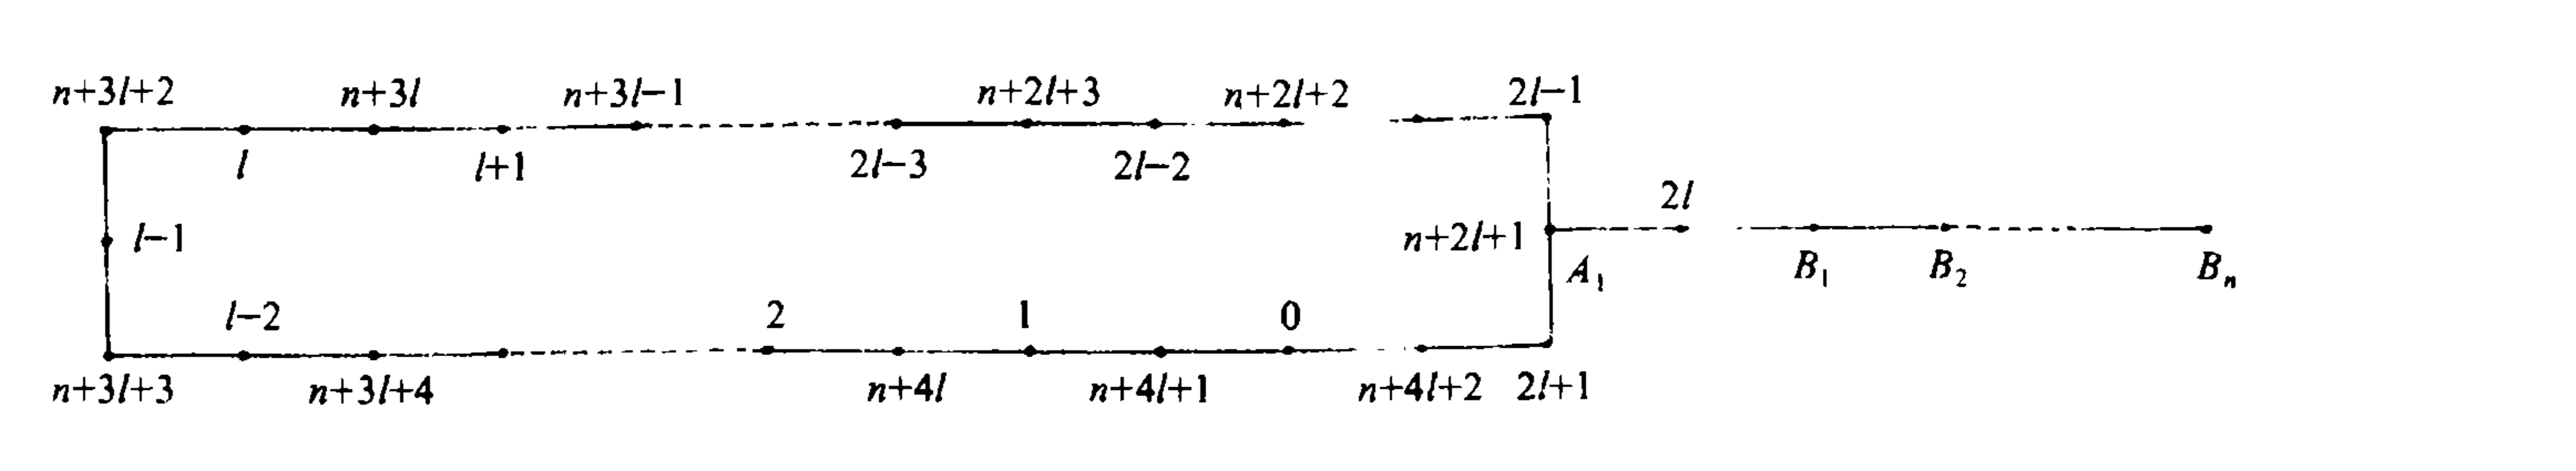
\includegraphics[width=\linewidth]{fig1.png}
  \parbox[c]{0.8\textwidth}{\captionof{figure}{Labeling for \(B(m, 1)\) when \(m \equiv 2 \pmod 4\)}}
  \label{fig1}
\end{center}
\end{minipage}


\vspace{0.5\baselineskip}
\pyfunction{../code/graceful_tadpoles.py}{fig1}



\subsection{Case 2: \(n = 2\)}
\label{sec:fig2}

\begin{minipage}{\textwidth}
\begin{center}
  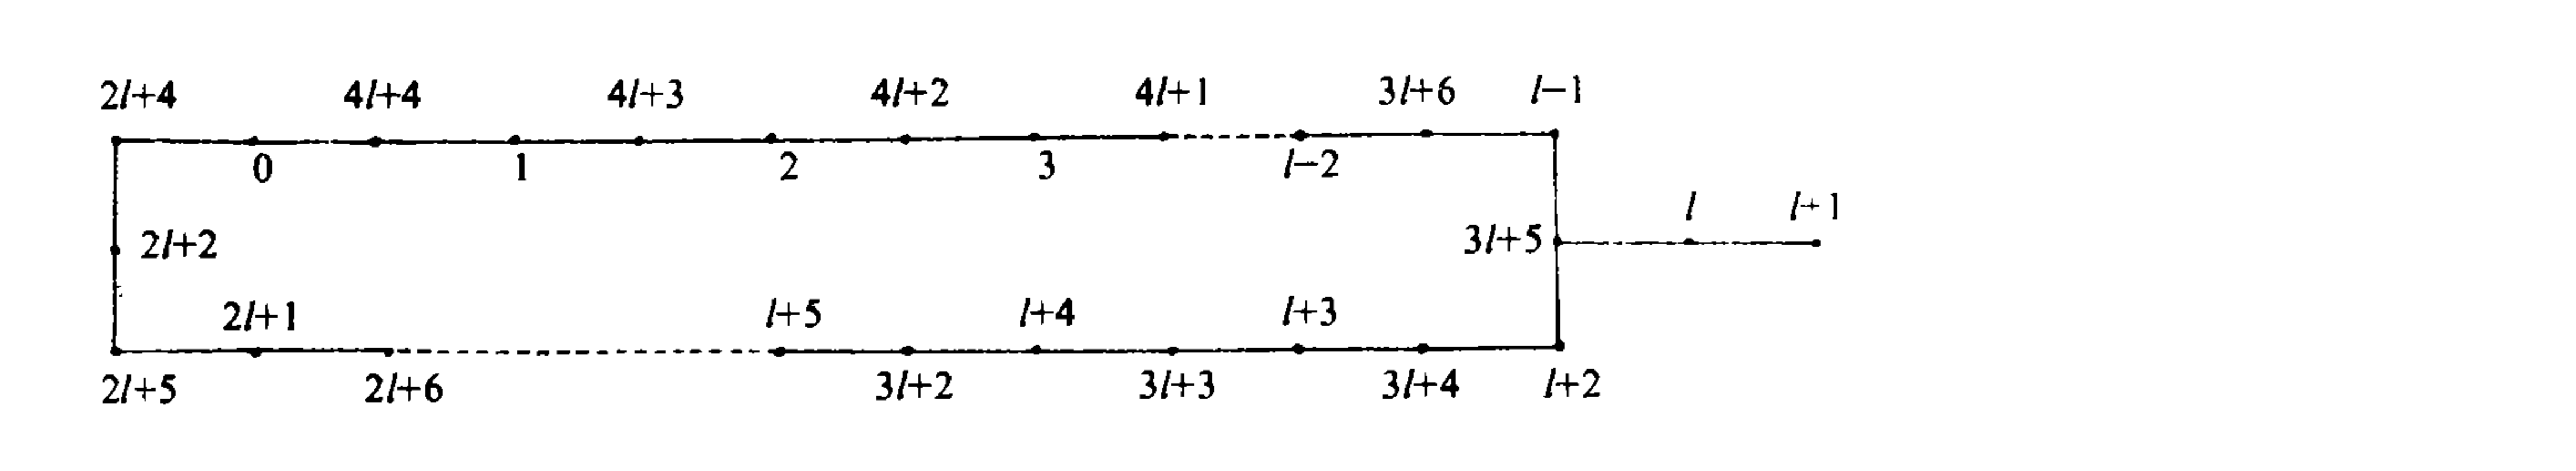
\includegraphics[width=\linewidth]{fig2.png}
  \parbox[c]{0.8\textwidth}{\captionof{figure}{Labeling for \(B(m, 2)\) when \(m \equiv 2 \pmod 4\)}}
  \label{fig2}
\end{center}
\end{minipage}

\pyfunction{../code/graceful_tadpoles.py}{fig2}

\subsection{Case 3: \(n \ge 3\)}\label{sec:restofthm1}
For the case \(n \ge 3\) we will construct graceful labelings as follows: 
  \begin{itemize}
  \item
    First, \(C_{m} \cup \{ B_{1} \} \) is labeled according to Figure 1.
  \item
    The vertex labels for \(C_{m} \cup \{B_{1}\} \) are distinct and their set is
    \(\{0, 1, \ldots, 2l + 1\} \cup \{n+2l+1, n+2l+2, \ldots, n+3l\} \cup \{n+3l+2, \ldots, n+4l+1, n+4l+2\}\).
  \item
    The edge labels are distinct and their set is
    \(\{n, n+1, \ldots, n+4l+1, n+4l+2\}\).
  \item
    The remaining path is \(B_{1}B_{2} \ldots B_{n}\), and the available edge label set is \(\{1, 2, \ldots, n-1\}\).
  \item
    The labeling for the path \(B_{1}B_{2} \ldots B_{n}\) is then given
    across six cases based on \(n \pmod 6\).
  \end{itemize}
% \end{enumerate}

\textbf{Labeling for Path \(B_{1}B_{2} \ldots B_{n}\) (for \(n \ge 3\))}

\begin{description}
  
\item[Case (3-1)] Let \(n=6s+3\),  \(a = \varphi(A_{1}) = n+2l+1\), and \(b = \varphi(B_{1}) = 2l\). The general assignments for \(0 \le i \le s-1\) are:
\begin{equation}
\label{eq:case31}
  \begin{aligned}
  \varphi(B_{6i+1}) &= b+3i   & \quad \quad 0 \leq i \leq s-1\\
  \varphi(B_{6i+2}) &= a-2-3i & \quad \quad 0 \leq i \leq s-1\\
  \varphi(B_{6i+3}) &= b+2+3i & \quad \quad 0 \leq i \leq s-1\\
  \varphi(B_{6i+4}) &= a-1-3i & \quad \quad 0 \leq i \leq s-1\\
  \varphi(B_{6i+5}) &= b+4+3i & \quad \quad 0 \leq i \leq s-1\\
  \varphi(B_{6i+6}) &= a-3-3i & \quad \quad 0 \leq i \leq s-1\\
  \varphi(B_{6s+1}) &= 2l+3s \\
  \varphi(B_{6s+2}) &= 2l+2+3s \\
  \varphi(B_{6s+3}) &= 2l+3+3s \\
  \end{aligned}
\end{equation}
It is easy to see that the labels are all distinct, and they consist of all integers from $2l$ to $2l+n$ with 
$2l+1$ removed, and the label of $B_1$ is still $2l$. Comparing with the set of labels on $C_m \cup A_1 \cup B_1$, we can conclude that the labels on $C_m \cup P_m$  are also all distinct, and do not exceed $|E|=n+m=n+4l+2$.
 
Calculating the number of edge labels, we have:
\begin{equation}
\label{eq:case31edges}  
\begin{aligned}
L(B_{6i+1}B_{6i+2}) &= n-1-6i \\
L(B_{6i+2}B_{6i+3}) &= n-3-6i \\
L(B_{6i+3}B_{6i+4}) &= n-2-6i \\
L(B_{6i+4}B_{6i+5}) &= n-4-6i \\
L(B_{6i+5}B_{6i+6}) &= n-6-6i \\
L(B_{6i+6}B_{6i+7}) &= n-5-6i
\end{aligned}
\end{equation}

Here $0 \leq i \leq s-1$. In the above six formulas, letting $i=0,1,\ldots,s-1$ respectively, we see that the edge labels are all distinct and form the $n-3$ edge labels from $3$ to $n-1$.

Moreover, since 
$L(B_{6s+1} B_{6s+2})=2$ and $L(B_{6s+2} B_{6s+3})=1$, it follows that the set of edge labels of $B_1,B_2,\ldots,B_n$ is $\{1,2,\ldots,n-1\}$.

Considering the case on $C_m \cup P_n$ as a whole, it is easy to see that the labeling method we give is graceful.

The proof for the other cases below is similar; we only present the key steps and omit the rest.

\vspace{0.5\baselineskip}
\pyfunction{../code/graceful_tadpoles.py}{case_3_1}

\item[Case (3-2)]
 When $n=6s+4$, the labels for $B_{1}$ to $B_{6s+1}$ still use formula (\ref{eq:case31}). 
 Additionally, we set:
\[
\begin{aligned}
\varphi(B_{6s+2}) &= 2l+3+3s \\
\varphi(B_{6s+3}) &= 2l+2+3s \\
\varphi(B_{6s+4}) &= 2l+4+3s \\
\end{aligned}
\]
The edge labels calculated by formula (\ref{eq:case31edges}) still apply, but the set of edge labels is now $\{4, 5, \ldots, n-1\}$. Furthermore, because
\[
L(B_{6s+1}B_{6s+2}) = 3, \quad L(B_{6s+2}B_{6s+3}) = 1, \quad L(B_{6s+3}B_{6s+4}) = 2, \text{ }
\]
Therefore, the set of edge labels for the path $B_{1}B_{2}\ldots B_{n}$ is $\{1, 2, \ldots, n-1\}$.

\vspace{0.5\baselineskip}
\pyfunction{../code/graceful_tadpoles.py}{case_3_2}

\item[Case (3-3)] 
When $n=6s+5$, the labels for $B_{1}$ to $B_{6s+1}$ still use formula (\ref{eq:case31}). Additionally, we set:
\[
\begin{aligned}
\varphi(B_{6s+2}) &= 2l+4+3s \\  
\varphi(B_{6s+3}) &= 2l+3+3s \\  
\varphi(B_{6s+4}) &= 2l+5+3s \\
\varphi(B_{6s+5}) &= 2l+2+3s \\ 
\end{aligned}
\]
The edge labels calculated by formula (\ref{eq:case31edges}) still apply, but the set of edge labels is now $\{5, 6, \ldots, n-1\}$. Furthermore, due to
\[
\begin{aligned}
L(B_{6s+1}B_{6s+2}) &= 4 \\
L(B_{6s+2}B_{6s+3}) &= 1 \\
L(B_{6s+3}B_{6s+4}) &= 2 \\
L(B_{6s+4}B_{6s+5}) &= 3 \\
\end{aligned}
\]
the set of edge labels for the path $B_{1}B_{2}\ldots B_{n}$ is $\{1, 2, \ldots, n-1\}$.

\vspace{0.5\baselineskip}
\pyfunction{../code/graceful_tadpoles.py}{case_3_3}

\item[Case (3-4)]
When $n = 6s + 6$, the labels for $B_{1}$ to $B_{6s+1}$ still use formula (1). Additionally, set:
\[
\begin{aligned}
\varphi(B_{6s+2}) &= 2l + 5 + 3s \\ 
\varphi(B_{6s+3}) &= 2l + 2 + 3s \\ 
\varphi(B_{6s+4}) &= 2l + 6 + 3s \\
\varphi(B_{6s+5}) &= 2l + 4 + 3s \\ 
\varphi(B_{6s+6}) &= 2l + 3 + 3s \\
\end{aligned}
\]
The edge labels calculated by formula (2) still apply, but the set of edge labels is now $\{6, 7, \ldots, n-1\}$. Furthermore, because
\[
\begin{aligned}
L(B_{6s+1}B_{6s+2}) &= 5 \\
L(B_{6s+2}B_{6s+3}) &= 3 \\
L(B_{6s+3}B_{6s+4}) &= 4 \\
L(B_{6s+4}B_{6s+5}) &= 2 \\
L(B_{6s+5}B_{6s+6}) &= 1 \\
\end{aligned}
\]
Therefore, the set of edge labels for the path $B_{1}B_{2}\ldots B_{n}$ is $\{1, 2, \ldots, n-1\}$.

\vspace{0.5\baselineskip}
\pyfunction{../code/graceful_tadpoles.py}{case_3_4}

\item[Case (3-5)] 
When $n = 6s + 7$, the labels for $B_{1}$ to $B_{6s+1}$ still use formula (1). Additionally, set:
\[
\begin{aligned}
\varphi(B_{6s+2}) &= 2l + 6 + 3s \\
\varphi(B_{6s+3}) &= 2l + 2 + 3s \\
\varphi(B_{6s+4}) &= 2l + 7 + 3s \\
\varphi(B_{6s+5}) &= 2l + 4 + 3s \\
\varphi(B_{6s+6}) &= 2l + 5 + 3s \\
\varphi(B_{6s+7}) &= 2l + 3 + 3s \\
\end{aligned}
\]

The edge labels calculated by formula (\ref{eq:case31edges}) still apply, but the set of edge labels is now $\{7, 8, \ldots, n-1\}$. 
Furthermore, because
\[
\begin{aligned}
L(B_{6s+1}B_{6s+2}) &= 6 \\
L(B_{6s+2}B_{6s+3}) &= 4 \\
L(B_{6s+3}B_{6s+4}) &= 5 \\
L(B_{6s+4}B_{6s+5}) &= 3 \\
L(B_{6s+5}B_{6s+6}) &= 1 \\
L(B_{6s+6}B_{6s+7}) &= 2 \\
\end{aligned}
\]
the set of edge labels for the path $B_{1}B_{2}\ldots B_{n}$ is $\{1, 2, \ldots, n-1\}$.

\vspace{0.5\baselineskip}
\pyfunction{../code/graceful_tadpoles.py}{case_3_5}

\item[Case (3-6)] When $n = 6s + 8$, the labels for $B_{1}$ to $B_{6s+1}$ still use formula (\ref{eq:case31}). Additionally, set:
\[
\begin{aligned}
\varphi(B_{6s+2}) &= 2l + 7 + 3s \\
\varphi(B_{6s+3}) &= 2l + 2 + 3s \\
\varphi(B_{6s+4}) &= 2l + 8 + 3s \\
\varphi(B_{6s+5}) &= 2l + 4 + 3s \\
\varphi(B_{6s+6}) &= 2l + 5 + 3s \\
\varphi(B_{6s+7}) &= 2l + 3 + 3s \\
\varphi(B_{6s+8}) &= 2l + 6 + 3s \\
\end{aligned}
\]
The edge labels calculated by formula (\ref{eq:case31edges}) still apply, but the set of edge labels is now $\{8, 9, \cdots, n-1\}$. Furthermore, because
\[
\begin{aligned}
L(B_{6s+1}B_{6s+2}) &= 7 \\
L(B_{6s+2}B_{6s+3}) &= 5 \\
L(B_{6s+3}B_{6s+4}) &= 6 \\
L(B_{6s+4}B_{6s+5}) &= 4 \\
L(B_{6s+5}B_{6s+6}) &= 1 \\
L(B_{6s+6}B_{6s+7}) &= 2 \\
L(B_{6s+7}B_{6s+8}) &= 3 \\
\end{aligned}
\]
Therefore, the set of edge labels for the path $B_{1}B_{2}\cdots B_{n}$ is $\{1, 2, \cdots, n-1\}$.

\vspace{0.5\baselineskip}
\pyfunction{../code/graceful_tadpoles.py}{case_3_1}

\end{description}

In all cases, the set of edge labels for the path
\(B_{1}B_{2} \ldots B_{n}\) is \(\{1, 2, \ldots, n-1\}\). By combining
this with the labels of \(C_{m} \cup A_{1}B_{1}\), the entire graph
\(C_{m} \cup P_{n}\) has a graceful labeling.
% \end{proof}

\section{\texorpdfstring{Case
\(m \equiv 1 \pmod 4\)}{Case m \textbackslash equiv 1 \textbackslash pmod 4}}\label{theorem-2-case-m-equiv-1-pmod-4}

\begin{theorem}
For all \(m \equiv 1 \pmod 4\) and \(n > 0\),
\(B(m,n)\) is a \textbf{graceful graph}.
\end{theorem}

\begin{proof}
Let \(m = 4l + 1\).
If $n$ is odd, we proceed as described in Section~\ref{sec3:odd}.
If $n$ is even, we distinguish three cases in Section~\ref{sec3:even}.
\end{proof}

\vspace{0.5\baselineskip}
\pyfunction{../code/graceful_tadpoles.py}{thm2}

\subsection{Case \(n\) is odd} % \(n \in N_{1}\) 
\label{sec3:odd}



\begin{minipage}{\textwidth}
\begin{center}
  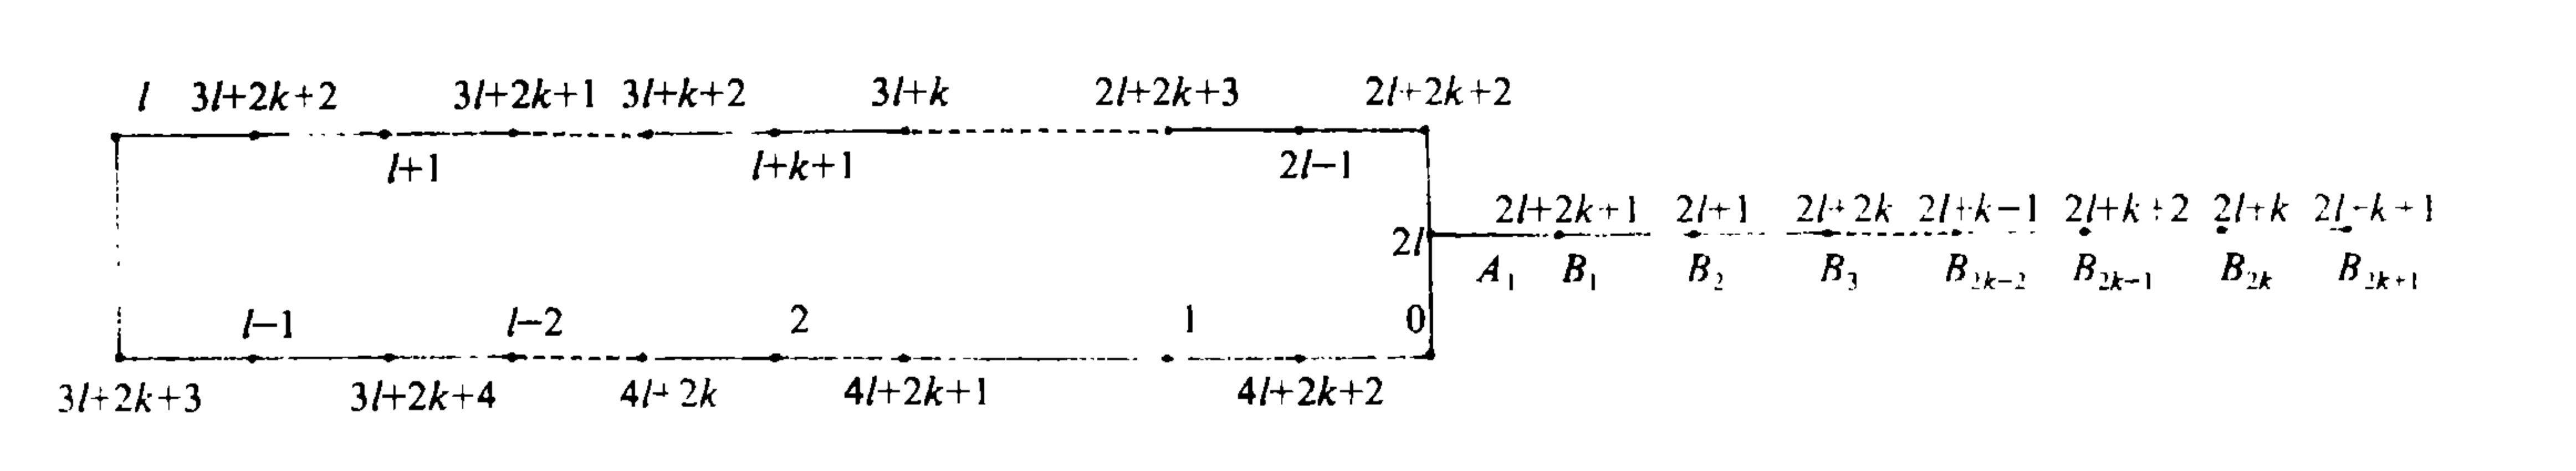
\includegraphics[width=\linewidth]{fig3.png}
  \parbox[c]{0.8\textwidth}{\captionof{figure}{Labeling for \(B(m, n)\) when
  \(m \equiv 1 \pmod 4\) and \(n=2k+1\) (odd, \(0 \le k \le l-2\))}}
  \label{fig3}
  \vspace{0.5\baselineskip}
\end{center}
\end{minipage}



% \begin{enumerate}
% \def\labelenumi{\arabic{enumi}.}
% \tightlist
% \item
  % \textbf{Case \(n \in N_{1}\) (\(n\) is odd)}: 
  Let \(n = 2k + 1\), where \(k\) is a non-negative integer.

  \begin{itemize}
  % \tightlist
  \item
    When \(0 \le k \le l-2\), a graceful labeling is given in Figure 3.
  \item
    When \(k > l-2\), the point labeled \(l+k+1\) in Figure 3 will be on
    the path \(A_{1}B_{1}B_{2} \ldots B_{2k+1}\).
  \end{itemize}

  \additionalcomment{
    The construction for this case labels the path $C_0C_2\ldots C_{m+n-1}$ with the node labels 
    \[ \varphi(C_i) = 
    \begin{cases}
      \frac{i}{2} & \text{ if $i$ is even } \\
      n+m - \frac{i-1}{2} & \text{ if $i$ is odd } \\
    \end{cases} 
    \]
    for $i < 2l+2k$ and 
    \[ \varphi(C_i) = 
    \begin{cases}
      \frac{i}{2} - 1 & \text{ if $i$ is even } \\
      n+m - \frac{i-1}{2} - 1 & \text{ if $i$ is odd } \\
    \end{cases} 
    \]
    for $i \geq 2l+2k$, skipping the edge label $2l$. This yields all edge labels $\{m, \ldots, 1\}$ in decreasing order, except $2l$. We note that $\varphi(C_{m-1}) = 2l$ and can hence connect $C_0$ and $C_{m-1}$ to obtain a graceful labeling for the tadpole $B(m, n)$.
    }

  \additionalcomment{
    Both variants are implemented in the \texttt{fig3} function.
  }
% \item

\vspace{0.5\baselineskip}
\pyfunction{../code/graceful_tadpoles.py}{fig3}


\subsection{Case \(n\) is even} % \(n \in N_{2}\) 
\label{sec3:even}
  % \textbf{Case \(n \in N_{2}\) (\(n\) is even)}: 
  Let \(n = 2k\), where \(k\) is a natural number.

  \begin{description}
  % \tightlist
  \item[Case (2-1)] 
  If \(k=1\) (\(n=2\)), a graceful labeling is given in Figure 4.

  \begin{minipage}{\textwidth}
  \begin{center}
    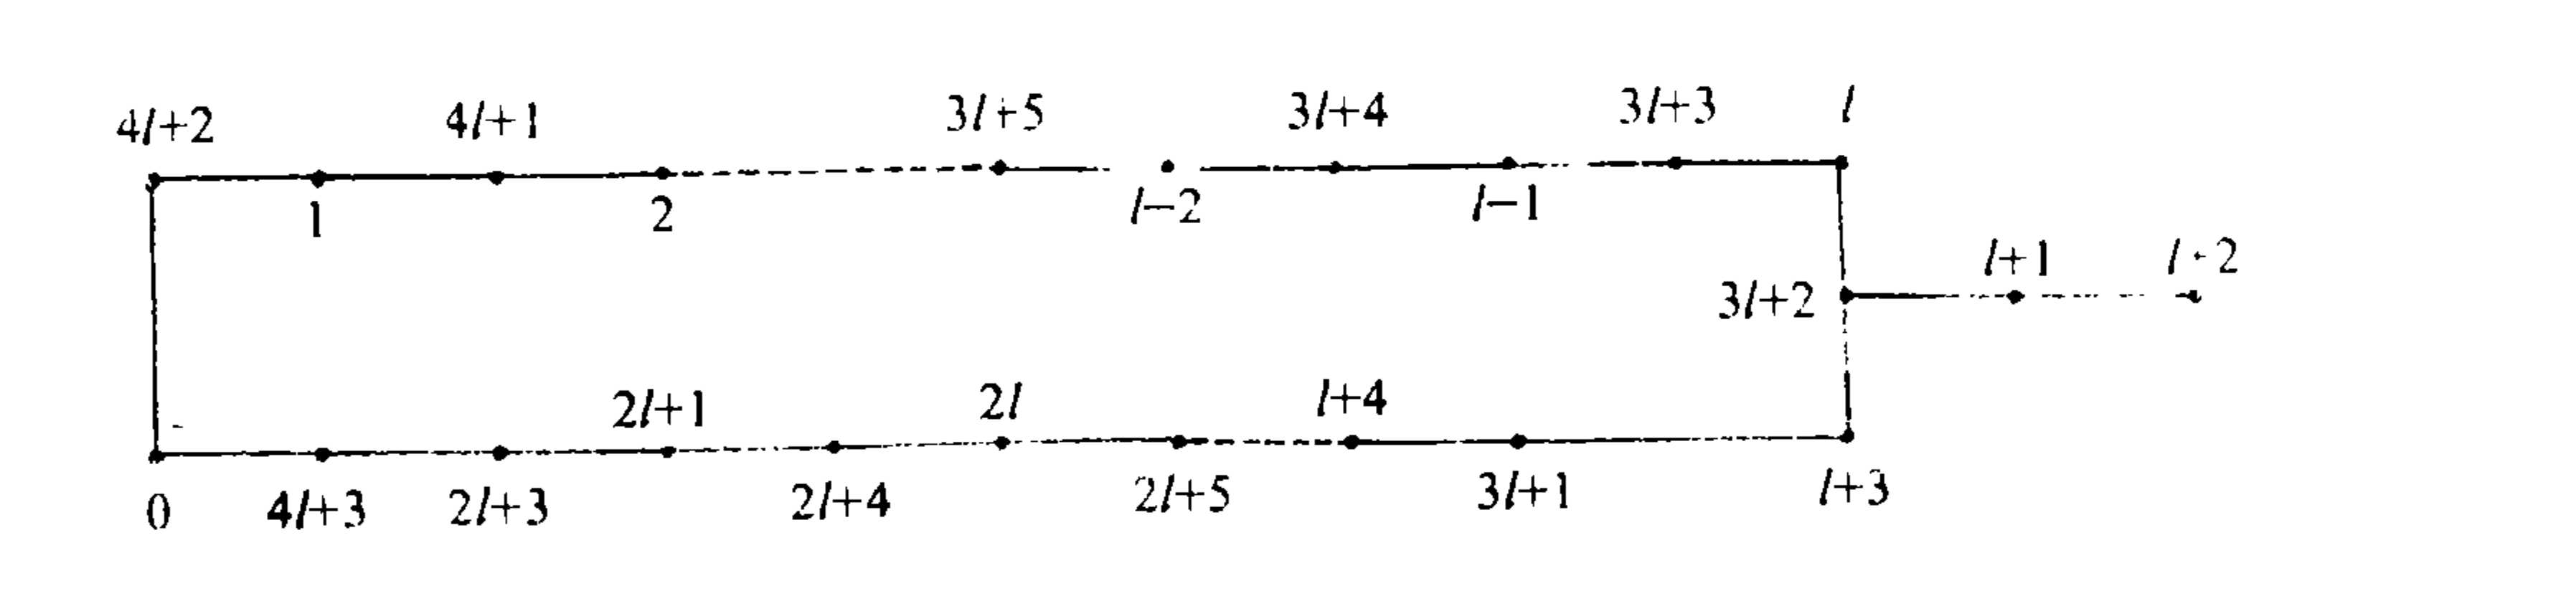
\includegraphics[width=\linewidth]{fig4.png}
    \parbox[c]{0.8\textwidth}{\captionof{figure}{Labeling for \(B(m, 2)\) when
    \(m \equiv 1 \pmod 4\) and \(n=2\)}}
    \label{fig4}
    \vspace{0.5\baselineskip}
  \end{center}
  \end{minipage}

  \vspace{0.5\baselineskip}
  \pyfunction{../code/graceful_tadpoles.py}{fig4}

  \item[Case (2-2)] 
  If \(k \ge l\) (\(k \ne 1\)), graceful labeling is given in Figure 5.
  
  \begin{minipage}{\textwidth}
  \begin{center}
    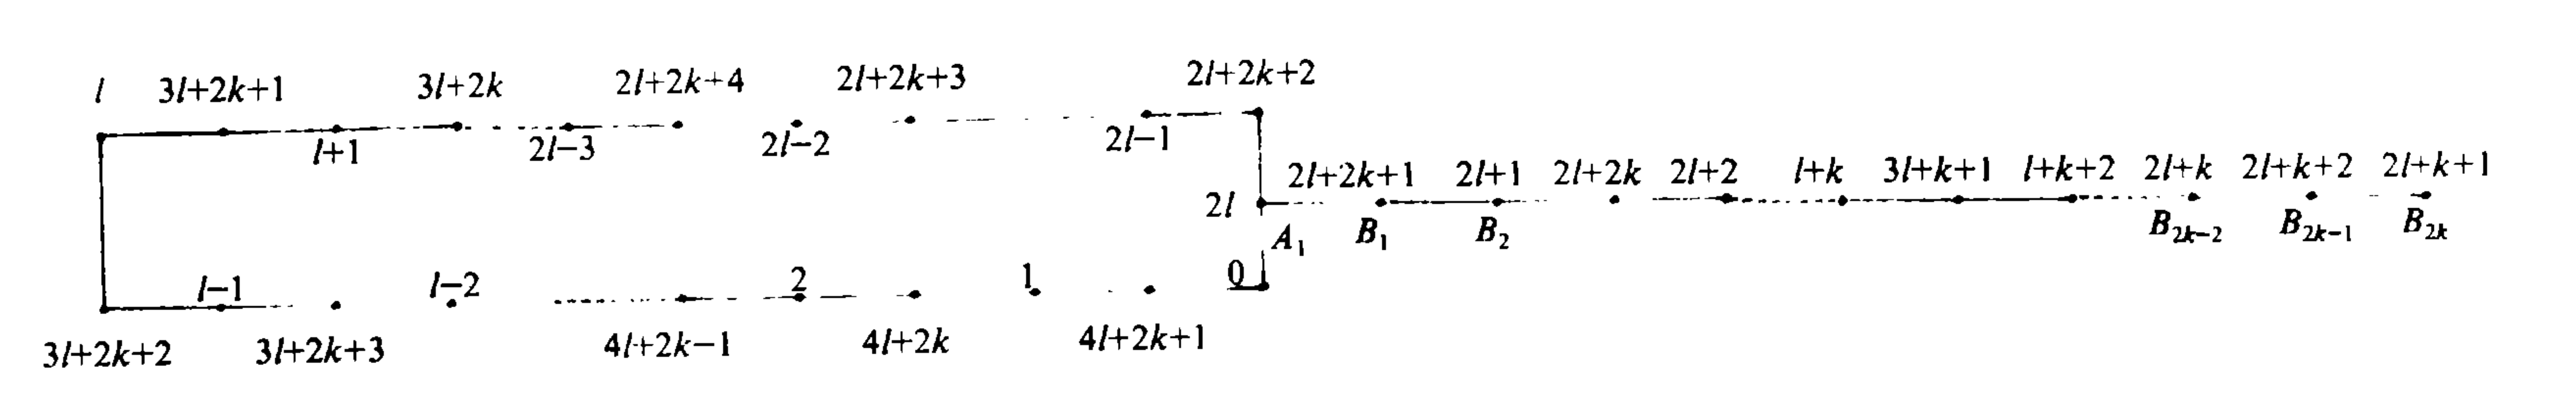
\includegraphics[width=\linewidth]{fig5.png}
    \parbox[c]{0.8\textwidth}{\captionof{figure}{Labeling for \(B(m, n)\) when
    \(m \equiv 1 \pmod 4\) and \(n=2k\) (even, \(k \ge l\))}}
    \label{fig5}
    \vspace{0.5\baselineskip}
  \end{center}
  \end{minipage}

  \vspace{0.5\baselineskip}
  \pyfunction{../code/graceful_tadpoles.py}{fig5}


  \item[Case (2-3)] 
  If \(1 < k < l\):

  \begin{minipage}{\textwidth}
  \begin{center}
    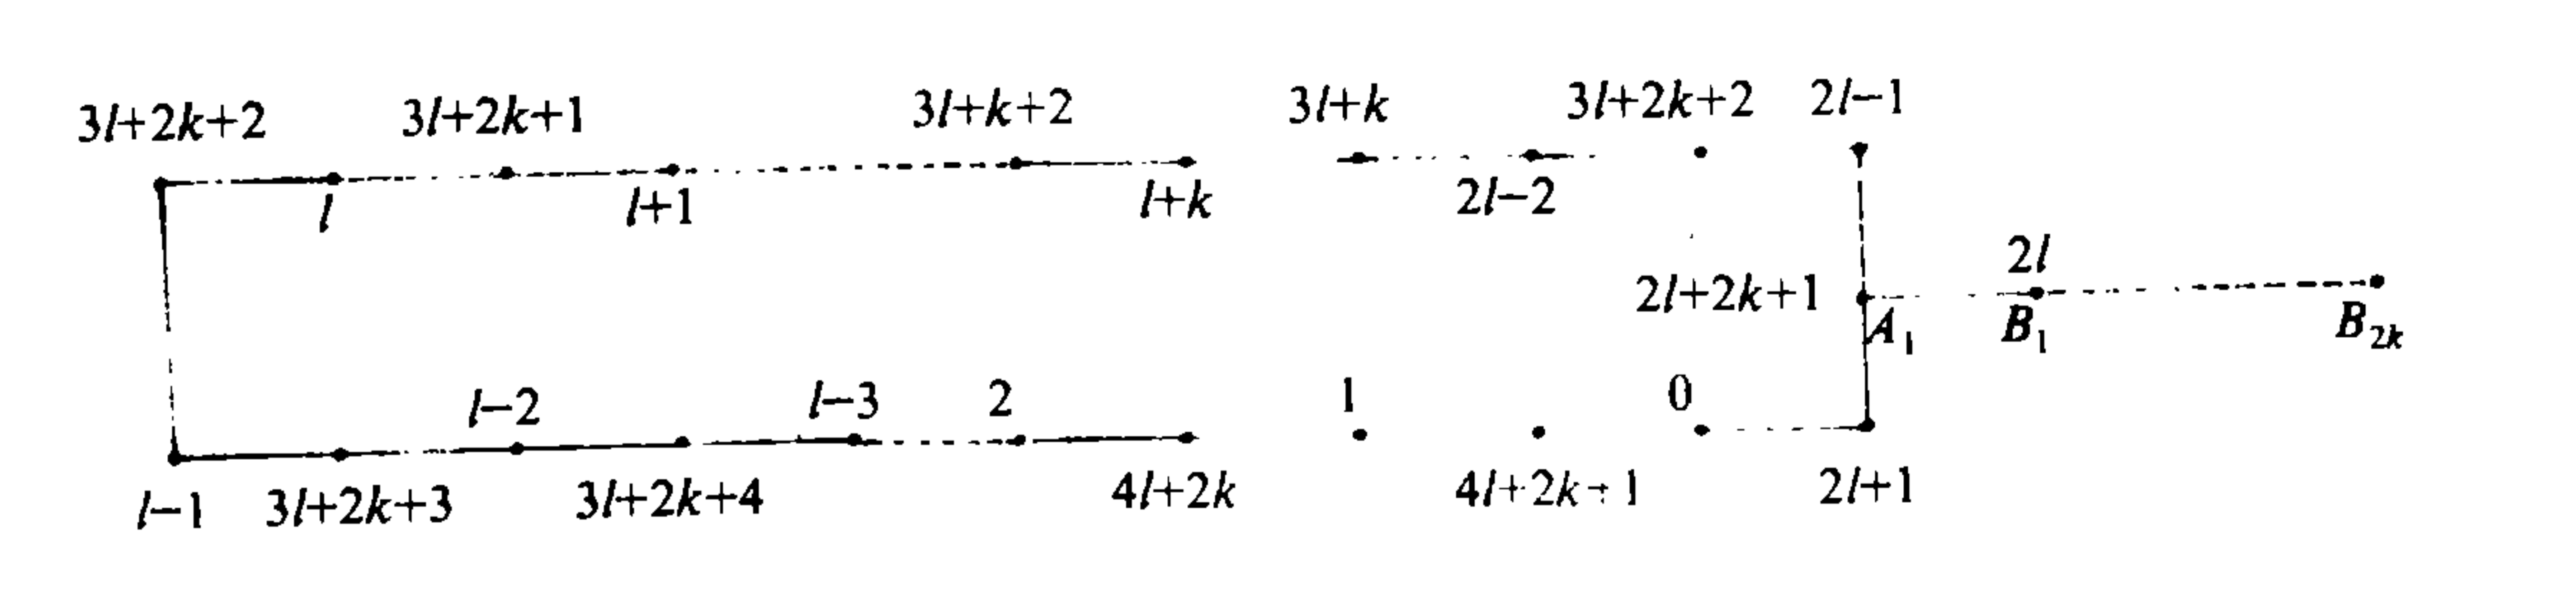
\includegraphics[width=\linewidth]{fig6.png}
    \parbox[c]{0.8\textwidth}{\captionof{figure}{Labeling for \(C_{m} \cup A_{1}B_{1}\) when \(m \equiv 1 \pmod 4\) and \(n=2k\) (even, \(1 < k < l\))}}
    \label{fig6}
    \vspace{0.5\baselineskip}
  \end{center}
  \end{minipage}

  \begin{itemize}
    % \tightlist
    \item
      First, \(C_{m} \cup A_{1}B_{1}\) is labeled according to Figure 6.
    \item
      The vertex label set for \(C_{m} \cup A_{1}B_{1}\) is
      \(\{0, 1, \ldots, 2l+1\} \cup \{2l+2k+1, \ldots, 3l+k\} \cup \{3l+k+2, \ldots, 4l+2k+1\}\).
    \item
      The edge label set is \(\{2k, 2k+1, \ldots, 4l+2k+1\}\).
    \item
      The remaining path is \(B_{1}B_{2} \ldots B_{n}\), and its
      required edge label set is \(\{1, 2, \ldots, 2k-1\}\).
    \item
      Since \(n\) is even, the construction methods from Theorem 1 for
      the even \(n\) cases---\textbf{(3-2)}, \textbf{(3-4)}, and
      \textbf{(3-6)}---can be used to give a graceful labeling for the
      remaining path.
    \end{itemize}
    \vspace{0.5\baselineskip}
    \pyfunction{../code/graceful_tadpoles.py}{fig6} 
    
  \end{description}
% \end{enumerate}
% \end{proof}

% \section{Figures (Illustrative
% Labelings)}\label{figures-illustrative-labelings}

% The paper references several figures (1 to 6) which provide the
% vertex labels for the graph \(B(m,n)\) in specific cases, demonstrating
% the existence of a graceful labeling.



% \begin{itemize}
% % \tightlist
% \item
%   \textbf{Figure 1}: Labeling for \(B(m, 1)\) when
%   \(m \equiv 2 \pmod 4\)
% \item
%   \textbf{Figure 2}: Labeling for \(B(m, 2)\) when
%   \(m \equiv 2 \pmod 4\)
% \item
%   \textbf{Figure 3}: Labeling for \(B(m, n)\) when
%   \(m \equiv 1 \pmod 4\) and \(n=2k+1\) (odd, \(0 \le k \le l-2\))
% \item
%   \textbf{Figure 4}: Labeling for \(B(m, 2)\) when
%   \(m \equiv 1 \pmod 4\) and \(n=2\)
% \item
%   \textbf{Figure 5}: Labeling for \(B(m, n)\) when
%   \(m \equiv 1 \pmod 4\) and \(n=2k\) (even, \(k \ge l\))
% \item
%   \textbf{Figure 6}: Labeling for \(C_{m} \cup A_{1}B_{1}\) when
%   \(m \equiv 1 \pmod 4\) and \(n=2k\) (even, \(1 < k < l\))
% \end{itemize}

\section{References}\label{references}
\begin{enumerate}
  \item\label{citeoriginal}
  Guo Wenfu. The Gracefulness of Graph $B(m,n)$. 
  Journal of Inner Mongolia Normal University (Natural Science Edition), 1994(2): 25-29.
  \item\label{cite1}
  Chen Zhizeng. On the $B(m,n,p)$ and $B(m,n)$ $3$-optimality. Journal of Inner Mongolia Normal University (Natural Science Edition), 1991(3): 11-19.
\end{enumerate}


\appendix

\section{Helper Functions}

\additionalcomment{To check if a constructed graph labeling is indeed graceful, i have written a test function. The python file contains a loop to check if the constructed labelings for tadpoles with $m \in \{3, \ldots, 1000\}$ and $n \in \{1, \ldots, 1000\}$ are indeed graceful. They are. :)} 

\vspace{0.5\baselineskip}
\pyfunction{../code/graceful_tadpoles.py}{is_graceful}

\section{Original Paper}
\label{apxoriginal}


\includepdf[pages=-]{original.pdf}

\end{document}